\documentclass[12pt]{article}
\usepackage{geometry}
\geometry{
	a4paper,
	top=2cm,
	bottom=2cm,
	left=2cm,
	right=2cm}
\usepackage[utf8]{inputenc}
\usepackage[english]{babel}
\usepackage{amsmath}
\usepackage{amssymb}
\usepackage{amsthm}
\usepackage[ruled,linesnumbered]{algorithm2e}
%\usepackage{graphicx}
\usepackage[usenames,dvipsnames]{xcolor}
\usepackage{color}
%\usepackage{graphicx}

\newcommand{\ass}{Robotic Systems\\ Report}
\newcommand{\name}{ Team: CJLZ-2\\Sergio Castillo-Hernández(jc15275)\\ Vince Jankovics (vj15292)\\ Miguel Lagunes-Fortiz(ml15765)\\ Kaiyang Zhou(kz15291)}

%\usepackage{natbib}
%\bibliographystyle{agsm}
%\usepackage[backend=bibtex,style=authoryear,sorting=nyt,maxcitenames=2,uniquelist=false]{biblatex}
\usepackage[backend=bibtex]{biblatex}
\addbibresource{ref.bib} % note the .bib is required


\usepackage{listings}
\lstset{language=matlab,tabsize=3,backgroundcolor=\color{light-gray}}
\lstset{commentstyle=\color{Sepia},numbers=left,stepnumber=5}
\lstset{keywordstyle=\color{MidnightBlue}\bfseries\emph,
stringstyle=\color{Mulberry},
numberstyle=\color{gray},
tabsize=2,
caption=\lstname,
breaklines=true,
identifierstyle=\color{Mahogany}}

\usepackage{enumitem}
\setlist{noitemsep} % or \setlist{noitemsep} to leave space around whole list


%\usepackage{cite}
\usepackage{hyperref}
\hypersetup{
 colorlinks,
 citecolor=Black,
 linkcolor=Black,
 urlcolor=Blue}
 
\usepackage{ifpdf}
\ifpdf
\usepackage[pdftex]{graphicx}
\graphicspath{{./fig/}}
\usepackage[outdir=./]{epstopdf}
\epstopdfDeclareGraphicsRule{.eps}{pdf}{.pdf}{%
ps2pdf -dAutoRotatePages/None -dEPSCrop #1 \OutputFile
}
\else
\usepackage{graphicx}
\fi
%\epstopdfDeclareGraphicsRule{.gif}{png}{.png}{convert gif:#1 png:\OutputFile}
%\AppendGraphicsExtensions{.gif}

\usepackage{pst-all} 



%\usepackage{tikz}
\usepackage{caption}
\usepackage{subcaption}
\usepackage{placeins}
%\usepackage{subfig}
\usepackage{float}

%\usepackage{fullpage}


\newcommand{\tab}{\hspace*{15pt}}

\definecolor{light-gray}{gray}{0.95}

\usepackage{fancyhdr}
\setlength{\headheight}{0pt}
\pagestyle{fancy}

%\renewcommand{\theenumi}{\alph{enumi}}

\newcommand{\vc}[1]{\mathbf{#1}}

%\renewcommand{\sectionmark}[1]{}
%\renewcommand{\chaptermark}[1]{}
%\renewcommand{\refname}{}
\renewcommand{\subsectionmark}[1]{}  
\renewcommand{\headrulewidth}{0pt}
\fancyhead{}
\rhead{}
\rfoot{}
\lhead{}

%\usetikzlibrary{calc}

\newcommand*{\titleM}{
\thispagestyle{empty}
\newlength{\drop}
\begingroup% Misericords, T&H p 153

%\begin{tikzpicture}[remember picture, overlay]
%    \node[inner sep=0pt] at (current page.center){%
%        \includegraphics[width=\paperwidth]{header6.png}%
%    };%
%\end{tikzpicture}

\drop = 0.18\textheight
\centering
\vspace*{\drop}
\vspace*{\drop}
{\Huge\bfseries \ass}\\[\baselineskip]
{\large\scshape \name}\par
\vfill
%\vspace*{2\drop}
%\pagebreak
\endgroup

\thispagestyle{empty}
\makebox[\textwidth]{}
\pagebreak
\makebox[\textwidth]{}
\setcounter{page}{0}
}

\newcommand{\figs}{0.9}
\newcommand{\dt}{\mathrm{d}t}
\newcommand{\der}[1]{\frac{\mathrm{d}#1}{\dt}}
\newcommand{\F}[1]{\mbox{Figure \ref{#1}}}
\newcommand{\comment}[1]{\textit{\textcolor{Green}{#1}}}
\newcommand{\question}[1]{\textit{\textcolor{Red}{#1}}}
\headsep = 25pt

\renewcommand{\qedsymbol}{$\blacksquare$}
%\setlength\itemsep{0em}
%\renewcommand{\thesubsection}{\Alph{subsection})}
\renewcommand{\c}[1]{\mathrm{c}\left(#1\right)}
\newcommand{\s}[1]{\mathrm{s}\left(#1\right)}
\newcommand{\atan}[1]{\mathrm{atan2}(#1)}
\newcommand\SmallMatrix[1]{{%
%  \footnotesize
  \scriptsize \arraycolsep=0.8\arraycolsep\ensuremath{\begin{bmatrix}#1\end{bmatrix}}}}

\makeatletter
\newcommand*{\rom}[1]{\expandafter\@slowromancap\romannumeral #1@}
\makeatother

\begin{document}
	\titleM
	
	\section*{Introduction}

``Kidnapped robot'' is a mobile robot localisation and navigation problem, where the goal is to estimate the location of the kidnapped robot within a known map and navigate it to a desired target position. This project aims to design an effective and efficient method to tackle this problem. To achieve the aim, this project was first conducted in a simulated environment in MATLAB and then the proposed method was applied to a real robot, which is a Lego NXT robot. The challenges of this project are: first, the only sensor used to help detect the environment is an imperfect ultrasonic sensor, which means the sensor readings are influenced by noises; second, the robot needs to explore an optimal path toward the target with less distance; third, the robot is required to be safely navigated to the target without any collision into walls.

This report presents the method we proposed to solve the ``Kidnapped robot'' problem. The structure of this report is organised as follows: in section \ref{sec:robot} we introduce the configuration of our Lego robot and the sensor calibration; in section \ref{sec:method} we describe our proposed method; the experimental results are illustrated in section \ref{sec:result}; a discussion summarising this project is given in section \ref{sec:discuss}.


		
	\section{Robot Design}
% describe the design
% what are the advantages
We mainly focus on two aspects when configuring the Lego robot, namely {\itshape \rom{1})} stability and {\itshape \rom{2})} feasibility. The complete configuration of the robot is visualised in Fig.\ref{fig:robotconfig}, where there are three images showing the front, side and back appearances of the robot respectively. 

The total height of the robot is approximately 18 cm. The width and length are 13 cm and 19.5 cm, respectively. This configuration ensures that the robot does not occupy too much space in the arena. The ultrasonic sensor is placed in the lower front with an approximate height of 6.5 cm and has a vision range of 180 degrees. A previous prototype with the sensor on the top and 360 degrees of freedom was tested but the wire connected to de brick interfered the sensor spin. A novel feature used in this design is the support device installed in the back as shown in Fig.\ref{fig:backrobot}, where two balls are positioned inside the two white slots to reduce the friction between the ground and the support device while rotating and moving. 

\begin{figure}[h]
\centering
  \begin{subfigure}{0.25\textwidth}
  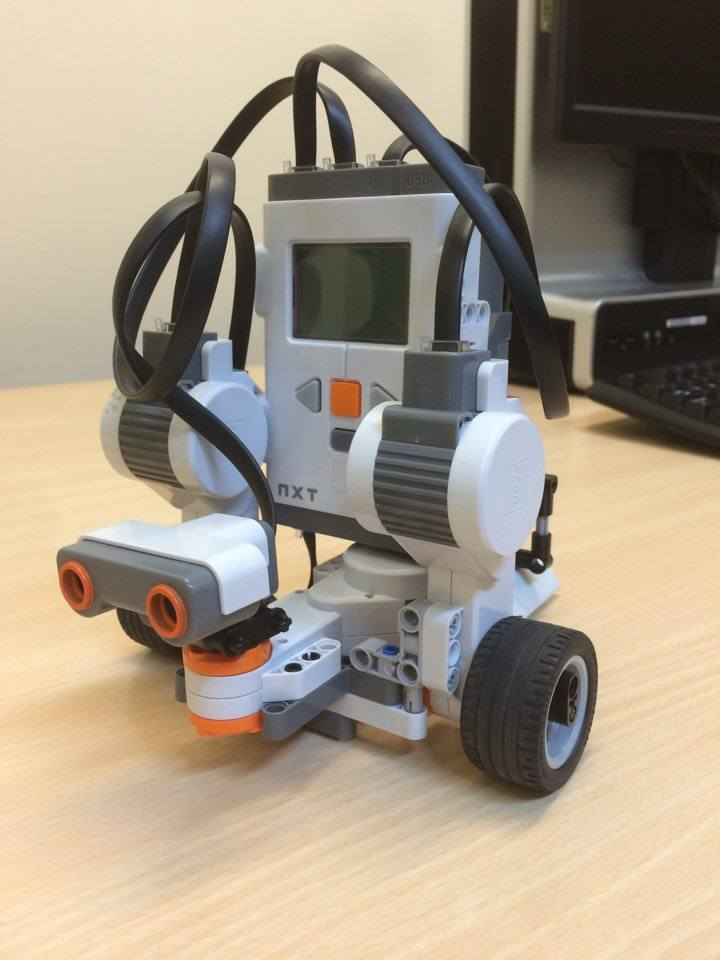
\includegraphics[scale=0.15]{f}
  \caption{Front appearance}
  \end{subfigure}
  \begin{subfigure}{0.25\textwidth}
  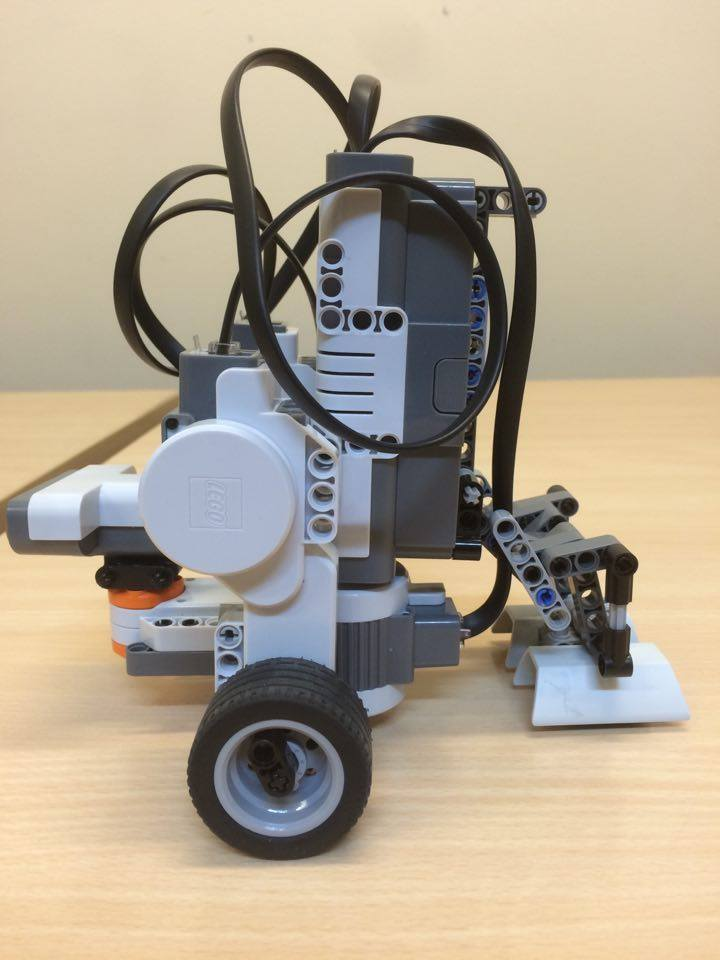
\includegraphics[scale=0.15]{s}
  \caption{Side appearance}
  \end{subfigure}
  \begin{subfigure}{0.25\textwidth}
  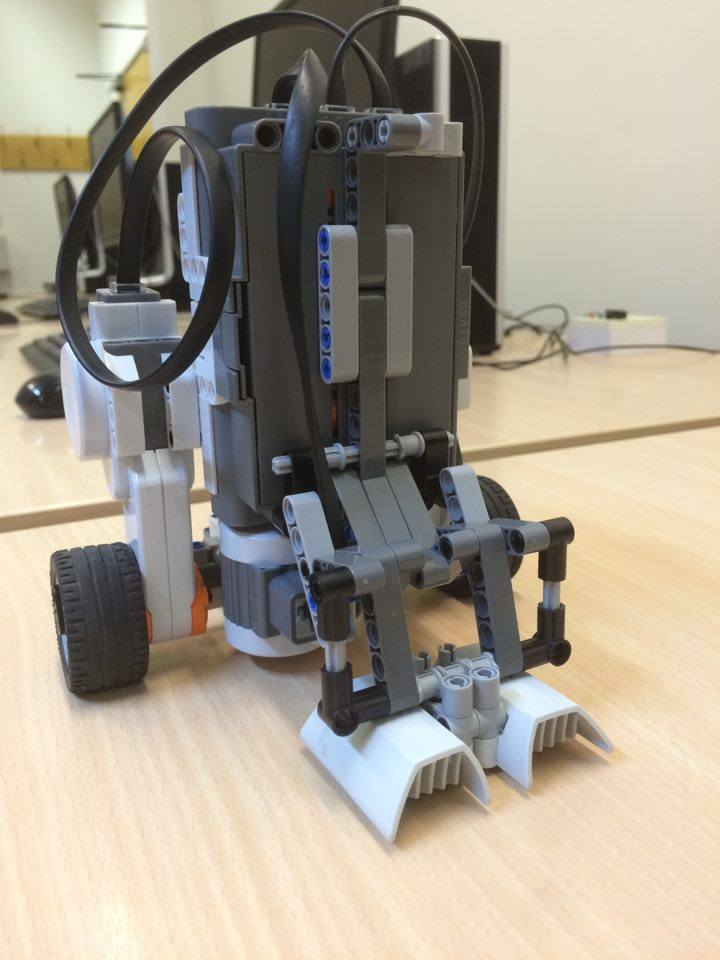
\includegraphics[scale=0.15]{b}
  \caption{Back appearance} \label{fig:backrobot}
  \end{subfigure}
  \caption{Robot configuration.}
  \label{fig:robotconfig}
\end{figure}

\FloatBarrier
 \label{sec:robot}
	
	
		
	\section{The kidnapped robot problem} \label{sec:method}
		
		
\subsection{Navigation}
In this section, we provide detailed implementation of particle filters localisation (PFL) and novel features used to boost the performance. The Bayesian reasoning of particle filters, however, is not focused in this section.

\vspace{1em}
\begin{algorithm}[H]
\caption{Particle filters localisation} \label{alg:pfl}
\SetAlgoLined
  \KwIn{particles, robot, isConverge}
  \KwOut{estimate, isConverge}  
  updateParticles(particles, robot); \\
  estimate = getEstimation(particles); \\
  \If{isConverge = true \label{alg:condition}}{
  \If{estimate is too different from real robot}{initialise particles; \\ isConverge = false;}
  }
  \Else{
  isConverge = checkConverge(particles); \\
  }
  \Return estimate, isConverge
\end{algorithm}
\vspace{1em}

% implementation details and novelty
We determine the size of particles as 400 via comprehensive experiments, which will be explained later. The implementation of PFL is demonstrated in Algorithm \ref{alg:pfl}. The input to this algorithm includes 400 particles, the real robot and a parameter called {\itshape isConverge} representing the status of these particles. When {\itshape isConverge} equals to 1, these particles are converged and 0 otherwise. The output of this algorithm contains two elements: first is the estimate of the real robot that contains estimated position and orientation; second is the status parameter that commands the robot to continue in exploring the environment to find its location or to move towards the target position.

Initially, the particles are positioned randomly inside a map. We add movement noise and turning noise to the particles using the given functions in the BotSim library. During the localisation process, we first update the particles in terms of their positions and orientations, which is enclosed in the function {\itshape updateParticles()}. To do so, firstly we obtain the scans (sensor readings) of the robot and the particles. These scans are represented as vectors $\mathbf{r}$ and $\mathbf{p}_{i}$, where $i = 1, ..., 400$, for the robot and particles respectively. Secondly, to update each particle's weights, we calculate the difference between the scan of the robot $\mathbf{r}$ and the scan of each particle $\mathbf{p}_{i}$ using the $\ell$1-norm i.e. $d_{i} = ||\mathbf{r} - \mathbf{p_{i}}||_{1}$, and then obtain the new weight for each particle by $$w_{i} = exp(-\frac{d_{i}}{2\sigma^{2}}) + damp$$ where $damp$ is a dampling factor used to prevent the weight from being zero. We use $\ell$1-norm instead of the $\ell$2-norm to compute the difference between two sensor readings because using $\ell$2-norm will make the weights of the particles less informative. For example, when using the $\ell$2-norm, each $d_{i}$ becomes much bigger since the difference is squared for each pair in the two vectors (sensor readings) and accordingly $exp(-\frac{d_{i}}{2\sigma^{2}})$ becomes much smaller and most of them are close to zero. As a consequence, all of the weights of the particles are nearly equal to the dampling factor, which makes the robot harder to match a particle. The $\sigma$ and $damp$ are assigned 3 and 0.01 respectively, which are obtained by running lots of experiments and selecting the optimal setting. Once the weights are computed, we normalise them by  $$w_{i} = \frac{w_{i}}{\sum_{i = 1}^{400}w_{i}} + \alpha$$ where $\alpha = 0.5/400$ is a constant. The reason for adding this constant will be explained later when we describe our resampling process.

The particles with larger weights are closer to the real robot. To do the resampling, we first resort the particles in a weight-decreasing order so the particle with the largest weight is positioned at the first and then we redistribute these particles. The particle with the max weight is copied for $n_{i} = w_{i}\times N$ times where $N=400$, and we repeat the same step for each particle in the queue until the number of the new particles is equal to 400 i.e. $\sum n_{i}=400$. However, during this process, we found that the number could not reach to 400 because many $n_{i}$ equaled to zero since $w_{i}\times N < 0.5$ (we used round to get an integer). Therefore, we add the constant $0.5/N$ to ensure the resulting $n_{i}$ satisfies $n_{i}\ge 0.5$ such that $n_{i}$ can be rounded to 1 rather than 0.

\begin{figure}[h]
\centering
  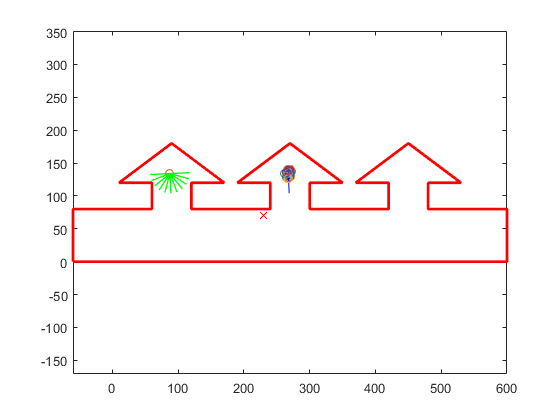
\includegraphics[scale=0.6]{symm}
  \caption{Robot in a symmetric environment causing the symmetric ambiguity problem.}
  \label{fig:symm}
\end{figure}

The {\itshape estimate} of the real robot that contains the position and orientation information is computed by separately averaging the positions and orientations of the new particles. After this, we check whether the particles were converged previously i.e. we go to Line \ref{alg:condition} in Algorithm \ref{alg:pfl}. There are two situations that will happen: (\textbf{1}) If they were converged, we need to check whether the obtained {\itshape estimate} matches the real robot or not. This step is necessary because if the map is somewhat symmetric as shown in Fig.\ref{fig:symm}, the particles were very likely to converge in a wrong place although the sensor readings were consistent with the robot's. We compare the {\itshape estimate} with the real robot in this way: suppose the sensor readings of the {\itshape estimate} are $\mathbf{e}$ and those of the real robot are $\mathbf{r}$, the difference between them is computed by $df=||\mathbf{e}-\mathbf{r}||_{1}$. If $df$ is bigger than a threshold, which means the {\itshape estimate} is inaccurate and the particles converged in an incorrect place, all the particles will be randomly positioned again and the status parameter {\itshape isConverge} will be set to {\itshape false}. (\textbf{2}) If the particles were not converged, they need to be checked by the function {\itshape checkConverge()}. With the observation that if the particles are converged, they will look compact in the 2D map. We thus use a statistical method to check the convergence: we calculate the 2 by 2 covariance matrix (CovMat) based on the positions $(x,y)$ of the particles and obtain the corresponding eigenvalues of the CovMat; these two eigenvalues describe the spread of the particles and how tight they are; we define the particles being converged if and only if the sum of the eigenvalues is lower than an experimentally determined threshold. By performing this localisation process, the particles are able to accurately find its location in a known map and the symmetric ambiguity is possible to be eliminated.

% how to select an optimal size
In order to select an optimal value as the size of the particle filters, we performed substantial experiments in which the size ranged from 100 to 1000 with an increment of 100. Thus there were totally 10 candidate values. We fixed the starting position of the real robot at $(20,20)$ and the target position at $(80,80)$ using the first map provided as shown in Fig.\ref{fig:experiment}. The distance between these two positions is sufficient for the particles to get converged. To judge the performance of the PFL with different size settings, we designed three criteria: {\itshape distance error} ($e$), {\itshape convergence time} ($t$) and {\itshape standard deviation} ($s$). The definitions of these three criteria are specified as follows:

\begin{itemize}
  \item Distance error ($e$): it is defined as the Euclidean distance between the target position and the final robot position.
  \item Convergence time ($t$): it calculates the time (in seconds) that the particles require to get converged.
  \item Standard deviation ($s$): it defines how accurate the estimated position is after the particles get converged and can represent the stability of the algorithm. The mathematical expression is as follows: suppose after the robot finds its location it requires $N$ steps to get stopped, denote the 2D position of the robot at each time step $i$ as $P^{r}_{i}$ and the estimation as $P^{e}_{i}$, the standard deviation $s$ is computed as $s = \sqrt{ \frac{1}{N}\sum_{i=1}^{N}||P^{r}_{i} - P^{e}_{i}||^{2} }$.
\end{itemize}

For each size setting, we ran 100 experiments where we computed the $e$, $t$ and $s$ for each and finally we averaged them as the output. The results are plotted in Fig.\ref{fig:sizedeter}, where the lower the values are, the better the performance is. It can be seen that the convergence time (green) increases as the size of the particle filters increases. On the distance error (blue) and the standard deviation (red), the algorithm with sizes from 300 to 1000 produces comparable results. Therefore, from this graph we could not decide which size is the optimal. To overcome this problem, we combined these three criteria to form a penalty-based criterion that can be used to distinguish one with the relatively best performance from the rest. We defined this criterion as {\itshape penalty-based score}, which was computed by $$psc = \frac{1}{e+1.5t+s}$$ The constant added before the $t$ aims to increase the weight of the convergence time such that the size that causes longer time for the particles to converge is less wanted since it decreases the score. As a result, the new ranking is more clear and the size equal to 400 has the best score as shown in Fig.\ref{fig:scorecompute}. Thesefore, we selected 400 as the optimal size.

% novel features
By running this algorithm to localise the robot in the simulation, we obtained promising results where the average distance from the target was always less than 3. Here we summarise the novel features used in this algorithm:

\begin{itemize}
  \item $\ell$1-norm based weights updating function.
  \item the $\alpha$ constant that is added when normalising the weights for the particles.
  \item a re-validation method to measure whether the obtained estimate is correct or not.
  \item a statistical method to determine the convergence condition.
  \item a penalty-based score to help select the optimal size for particle filters.
\end{itemize}

\begin{figure}[h]
\centering
  \begin{subfigure}{0.48\textwidth}
  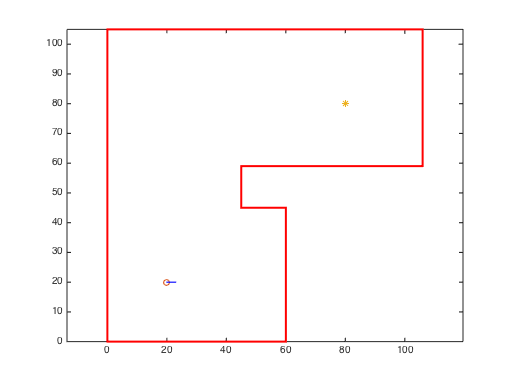
\includegraphics[scale=0.5]{experiment}
  \caption{}
  \label{fig:experiment}
  \end{subfigure}
  \begin{subfigure}{0.48\textwidth}
  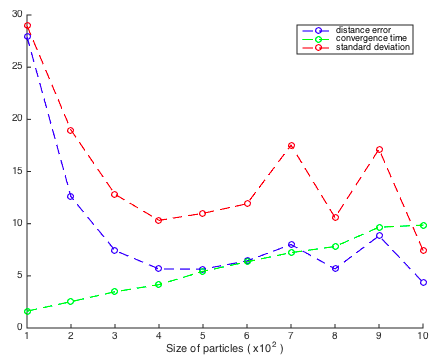
\includegraphics[scale=0.5]{sizedetermine}
  \caption{}
  \label{fig:sizedeter}
  \end{subfigure}
  \begin{subfigure}{0.48\textwidth}
  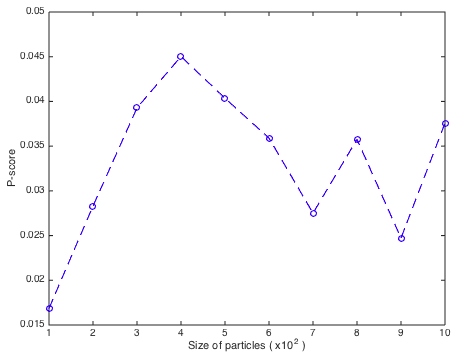
\includegraphics[scale=0.5]{scorecompute}
  \caption{}
  \label{fig:scorecompute}
  \end{subfigure}
  \caption{Experiments to select an optimal size of particle filters.}
\end{figure} 


\FloatBarrier
		
		
	For implementing the Particle weighting,  we considered two approaches for comparing the distance measurements from the robot (r) and particles (z):
	
		\begin{enumerate}
			\item Comparing every reading from the sensor individually, so the \textit{posterior} is the product of subtracting each sensor beams as showed on Algorithm 1. 
			\item Comparing the whole vector of readings by adding up the individual readings and then subtracting the scalar number as showed on Algorithm 2:
		\end{enumerate}
	
		\vspace{1em}
		\begin{algorithm}[H]
			\caption{Method 1 for Comparing distance reading} \label{alg:method2}
			... \\
			initialise weigths; \\
			botScan = robot.ultraScan(); \\
			
			\For{$particle \in  particles$} {
				pScan = (particle.ultraScan());\\
				prob=1;\\ 
				\For{$reading \in  particle$} {
					delta =  abs(robotBeamReading - particleBeamReading)\\
					prob = prob * exp( - delta / (2 * sigma*sigma) ) ;}
				weights(i) = prob+damping;}
			...\\
		\end{algorithm}
		\vspace{1em}
			
	
		\vspace{1em}
		\begin{algorithm}[H]
			\caption{Method 1 for Comparing distance reading} \label{alg:method1}
			... \\
			initialise weigths; \\
			botScan = robot.ultraScan(); \\
	 
			\For{$particle \in  particles$} {
				pScan = (particle.ultraScan());\\ 
				delta = sum( abs(pScan - botScan) );\\
				weights(i) = exp( - delta / (2 * sigma * sigma) ) + dampling;}
			...\\
		\end{algorithm}
		\vspace{1em}
	
	We tested both approaches by running the particle filter 500 times on the first map  and measured the convergence time and the distance error. We present the results on (Figure \ref{fig:methods}), we can infer that method one is slightly slower (2.91s vs 2.04s) but more accurate (1.88 cm vs 4.9 cm); however, method 1 is less robust to noisy data since a big difference in one beam can heavily penalise the whole particle, thus we used the method number 2 for further experiments and implementation. 
	

	\begin{figure}[h]
		\centering
		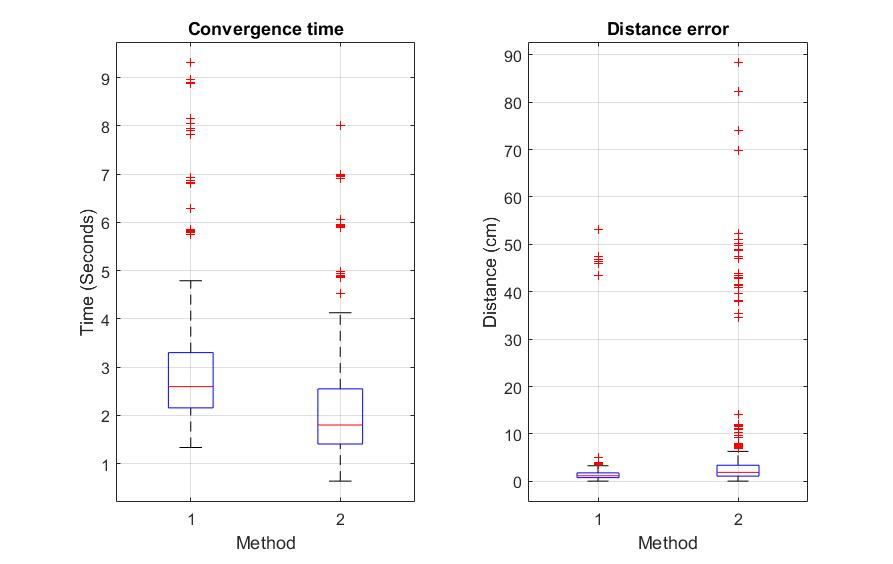
\includegraphics[width=.75\textwidth]{methods}
		\caption{Two approaches for comparing sensor data between the robot and its particles}
		\label{fig:methods}
	\end{figure}
	
	
	
	After finding the optimal number of particles, we aimed for finding an adequate number of beams for the sensor reading towards an accurate and fast implementation.
	
	On the simulation, we let the robot localise itself into the first map and we measured the convergence time of the particle filter and the distance error relative to the actual robot's position, we vary the number of beams from 5 to 40 using increments by 5 and running each experiment 500 times. 
	
	We present the results on (Figure \ref{fig:NumBeams}) and we  inferred that more sensor beams leads to a more accurate pose's estimation but also increases the computational time for convergence since more operations are required. Thus, we select 10 beams as an adequate value since offers both accuracy (mean error of 1.44cm) and fast computation time ( mean 3.34 seconds for convergence).  
	
	\begin{figure}[h]
    \centering
		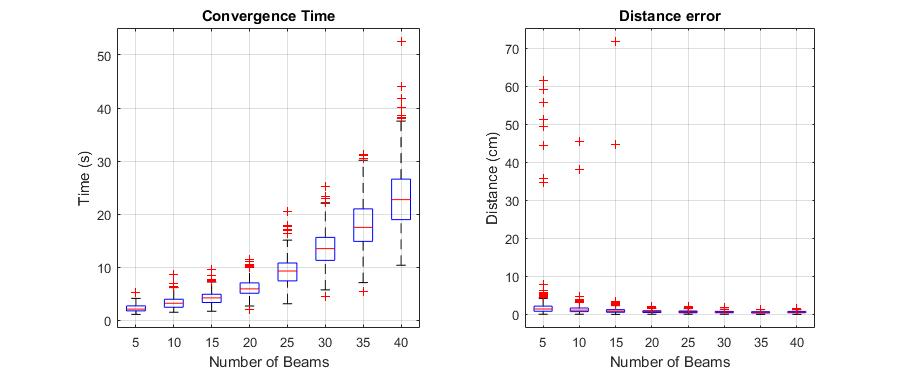
\includegraphics[width=.75\textwidth]{NumberOfBeams}
      \caption{Selecting an adequate number of sensor beams}
    \label{fig:NumBeams}
 	\end{figure}
	
	
	 

	
	
		
		\subsection{Guidance}

	Before and after the robot is localized in the map, it has to know what to do next according to the current objective, which are:
	\begin{enumerate}
		\item Avoid collision all time,
		\item Explore map,
		\item Go to target.
	\end{enumerate}
	
	\subsubsection{Collision avoidence}
	
		The robot's highest priority objective is avoiding collisions with the walls. This is done by a simple algorithm, which estimates the smallest distance between the robot and the scanned points based on the commanded movement. If this predicted distance is smaller than a certain threshold, it 'bounces back' from the boundary (see Figure \ref{fig:ca}). The reflected angle is perturbed with a small noise factor, so the robot does not get stuck in an area (e.g. when it goes perpendicular to the wall).
		
		\begin{figure}[h]
		   \centering
			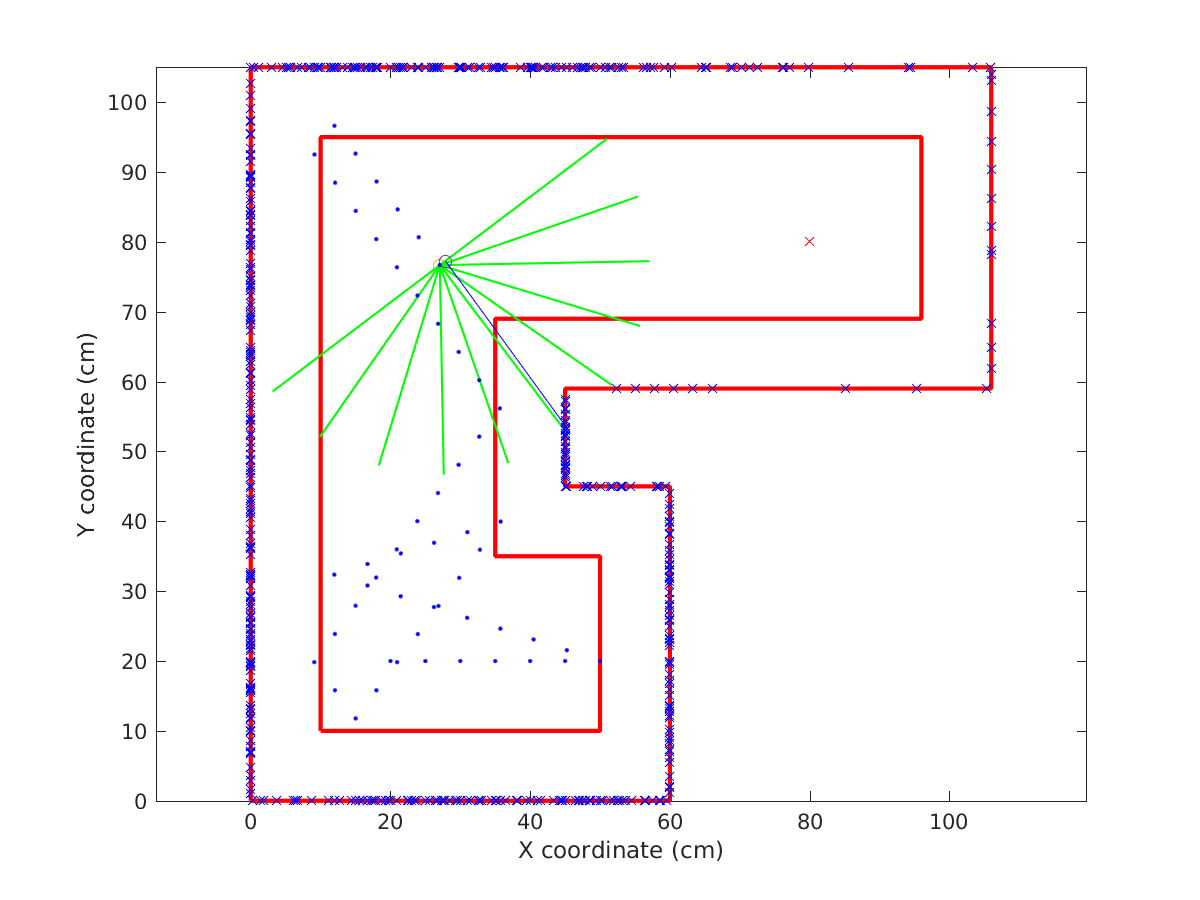
\includegraphics[width=.75\textwidth]{ca1}
		    
		   \caption{'Wall bouncing', with a distance threshold of 10cm (inner boundary).}
		   \label{fig:ca}
	 	\end{figure}
	
	\subsubsection{Exploration}
	
		The exploration is done before the PFL is converged to a location (i.e. the localization is not complete), so the robot can wonder around the map and exploit more of its features. The robot builds an internal map of the sensed points (called {\tt knownPoints} in the code) and the points where it had been (called {\tt beenThere} in the code), which serve as the basis of the decision making. These are based on the commanded movements and sensor data, so they are a rough estimate of the surrounding space. 
		
		The points are used to build an \textit{Artificial potencial field} ($U$), and drive the robot downhill (i.e. $-\nabla U$) \parencite{choset_principles_2005}. Since the points where the robot had been is also used for this field (with different weight than the walls), the robot is driven towards unexplored locations. The result can be seen on Figure \ref{fig:apf}.
		
		\begin{figure}[h]
		    \centering
		    \begin{subfigure}[b]{0.48\textwidth}
   	 			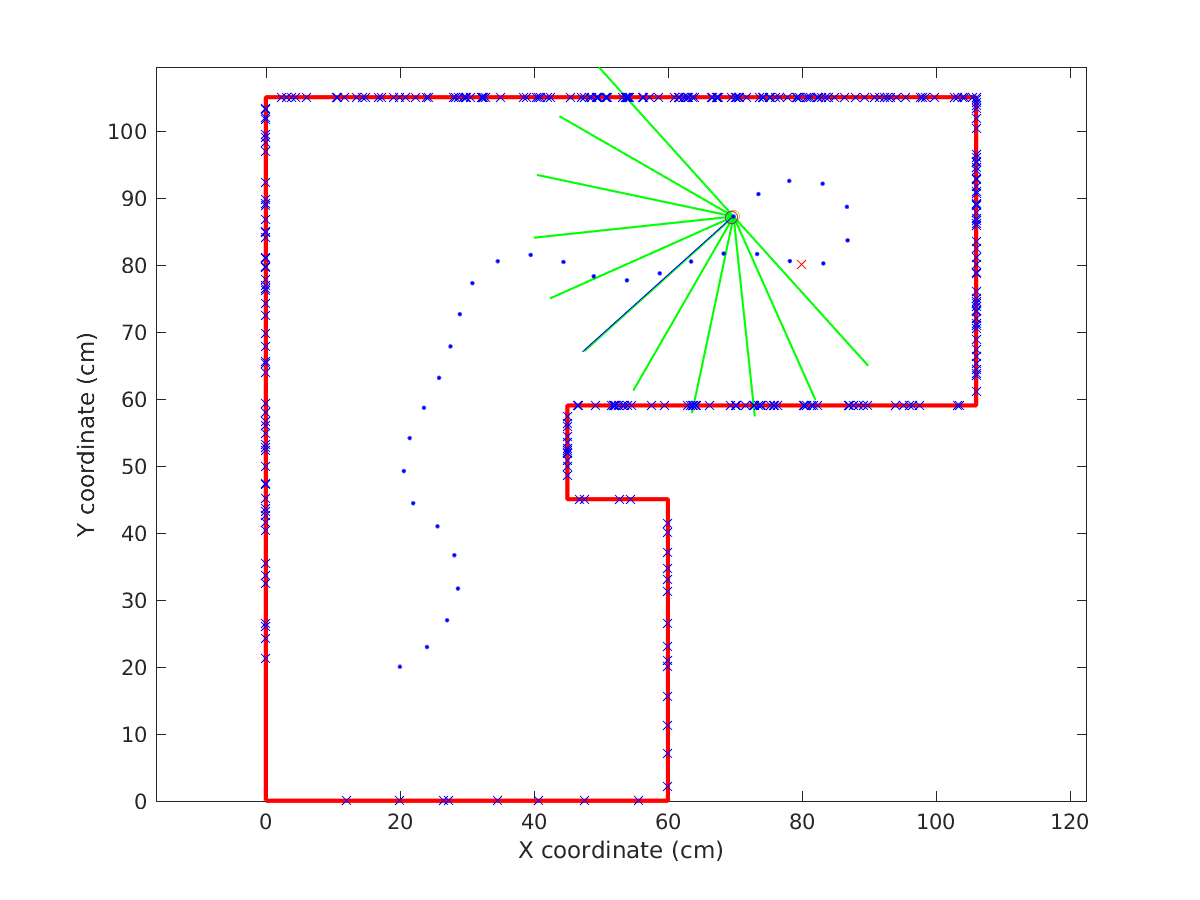
\includegraphics[width=\textwidth]{apf1}
   	 			\caption{}
				\label{fig:apf1}
   	 		\end{subfigure}		    
		    ~
		    \begin{subfigure}[b]{0.48\textwidth}
   	 			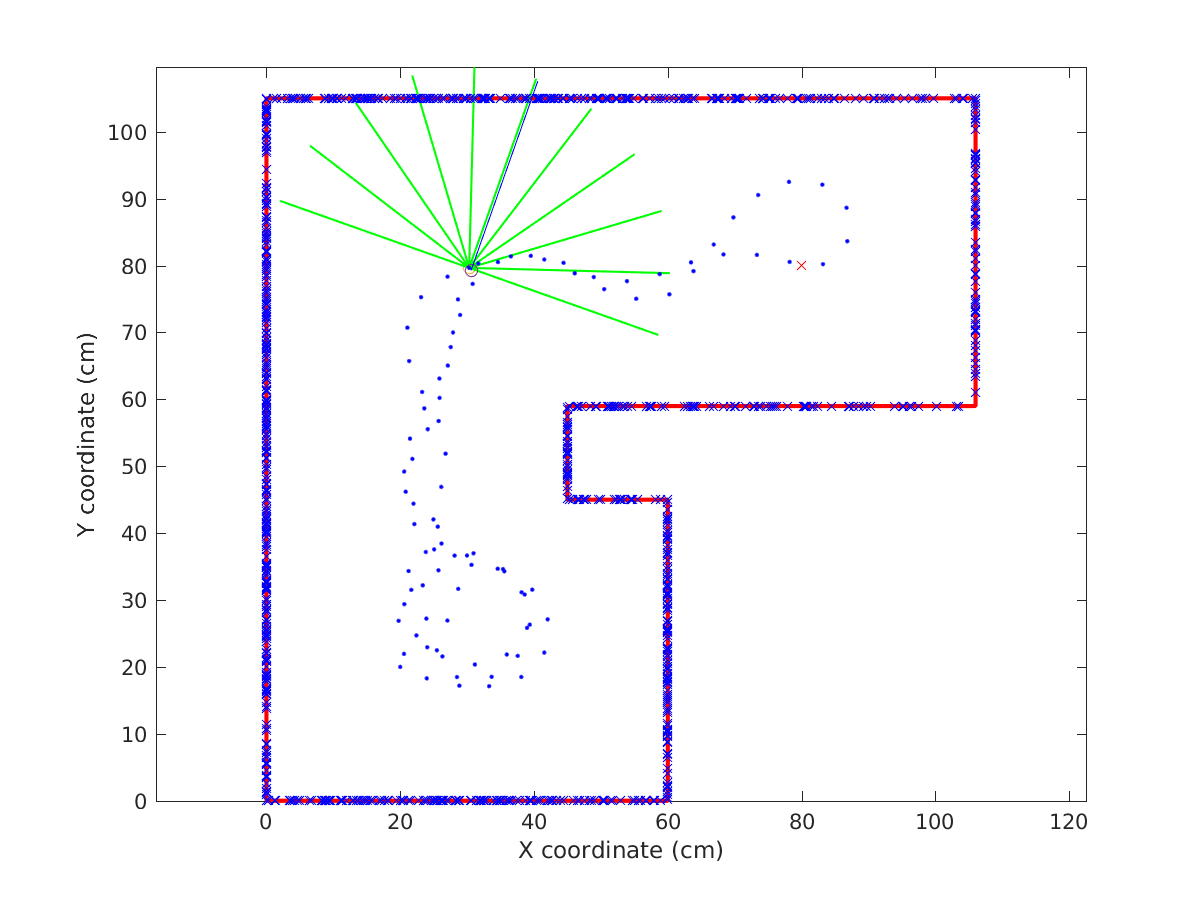
\includegraphics[width=\textwidth]{apf2}
   	 			\caption{}
 				\label{fig:apf2}
   	 		\end{subfigure}
   	 		%		    \subfloat[][]{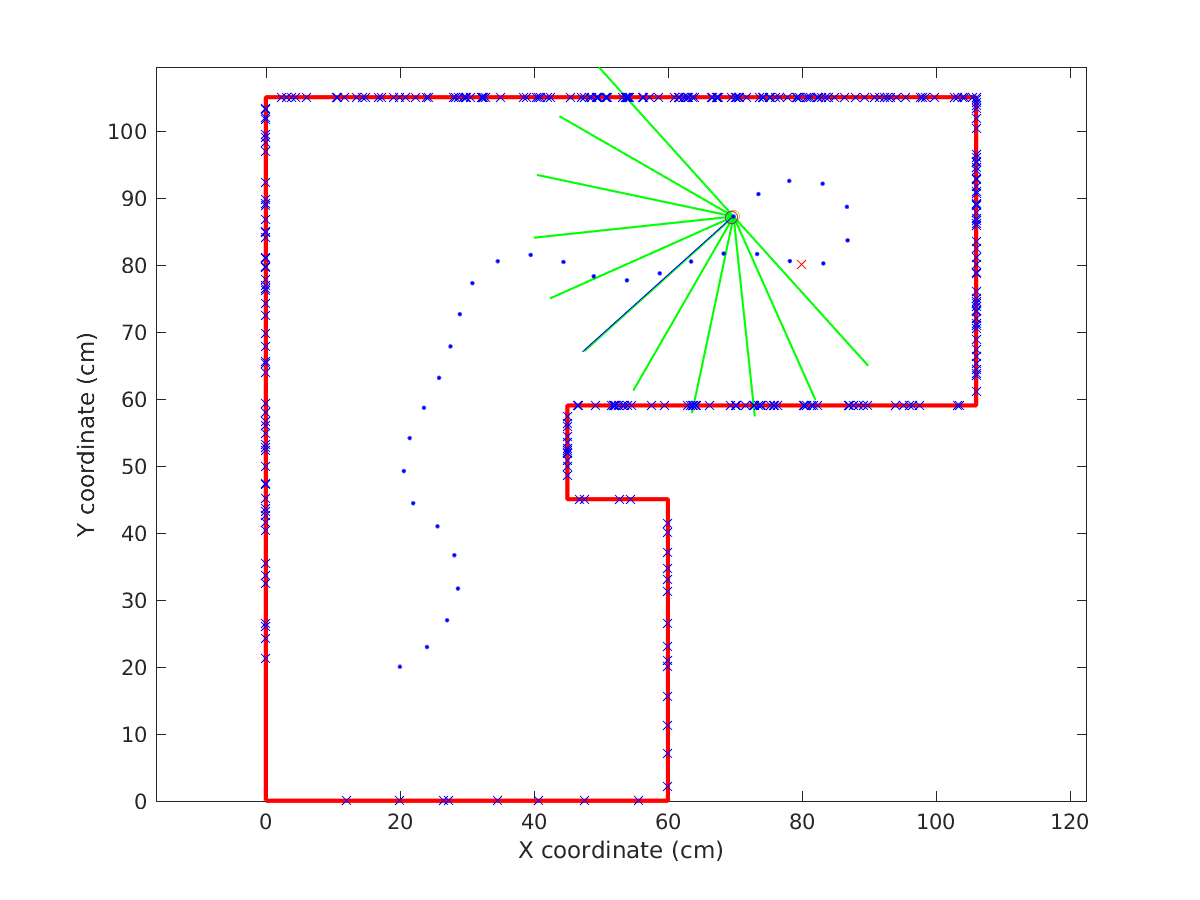
\includegraphics[width=.5\textwidth]{apf1}\label{fig:apf1}}
%		    \subfloat[][]{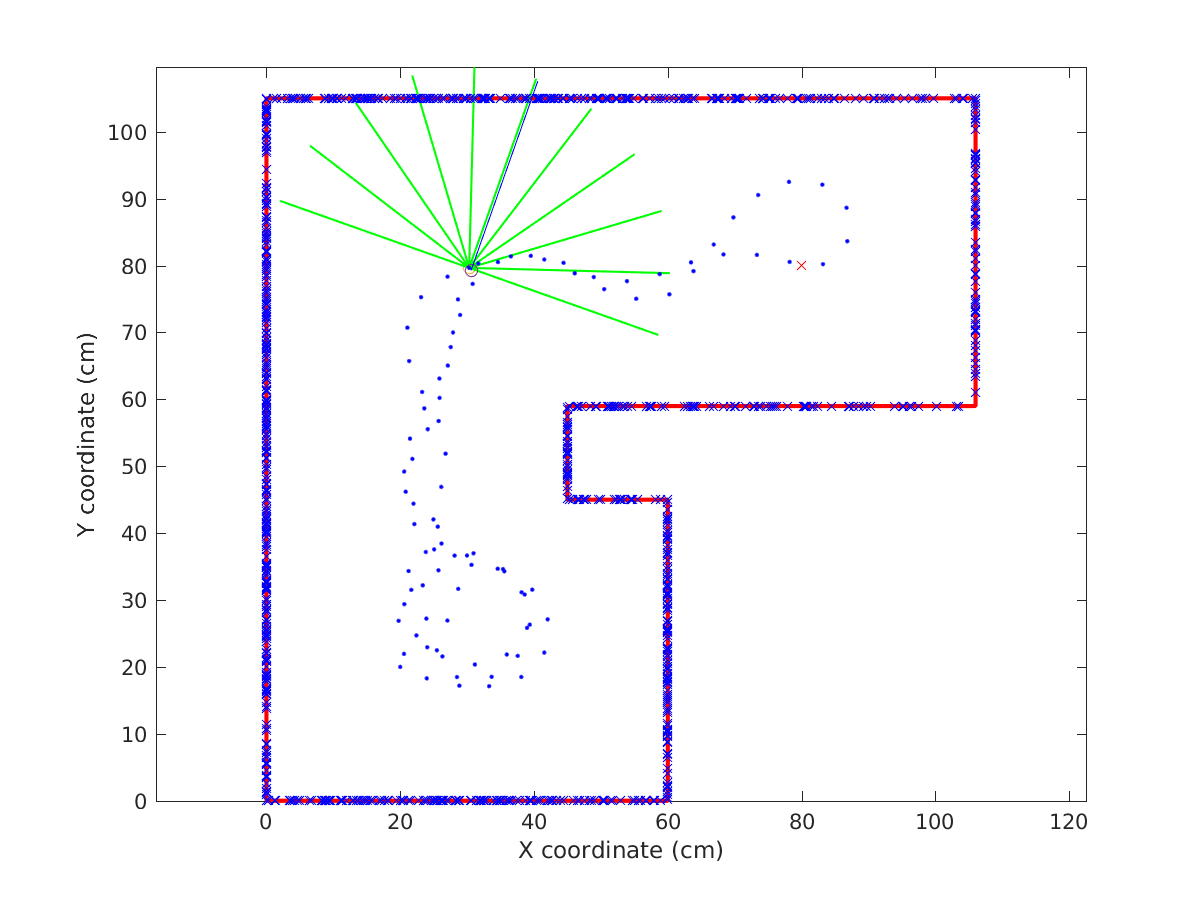
\includegraphics[width=.5\textwidth]{apf2}\label{fig:apf2}}
		     
		    \caption{Simulation with artificial potential field as guidance ($\epsilon=0.3$). (\protect\subref{fig:apf1}) Initial path. (\protect\subref{fig:apf2}) Path after some time.}
		    \label{fig:apf}
	 	\end{figure}
	 	
	 	
	 	
	 	The effect of the potencial field can be tuned by the constant $\epsilon$, so the commanded turning angle is:
	 	\begin{equation}
			\delta \theta=\epsilon\cdot\arg(-\nabla U),
	 	\end{equation}
	 	meaning that with lower $\epsilon$ the robot has higher inertia (goes more uphill). The commanded forward movement is kept constant, so the robot gives more consistent response even on higher gradient values (e.g. close to a wall).
	 	
	 	
	 	This feature improves the robot's movement compared to the simple bouncing, but it needs the collision avoidance as a simple backup. The result is shown on Figure \ref{fig:apf3}.

		
		\begin{figure}[h]
			\centering
			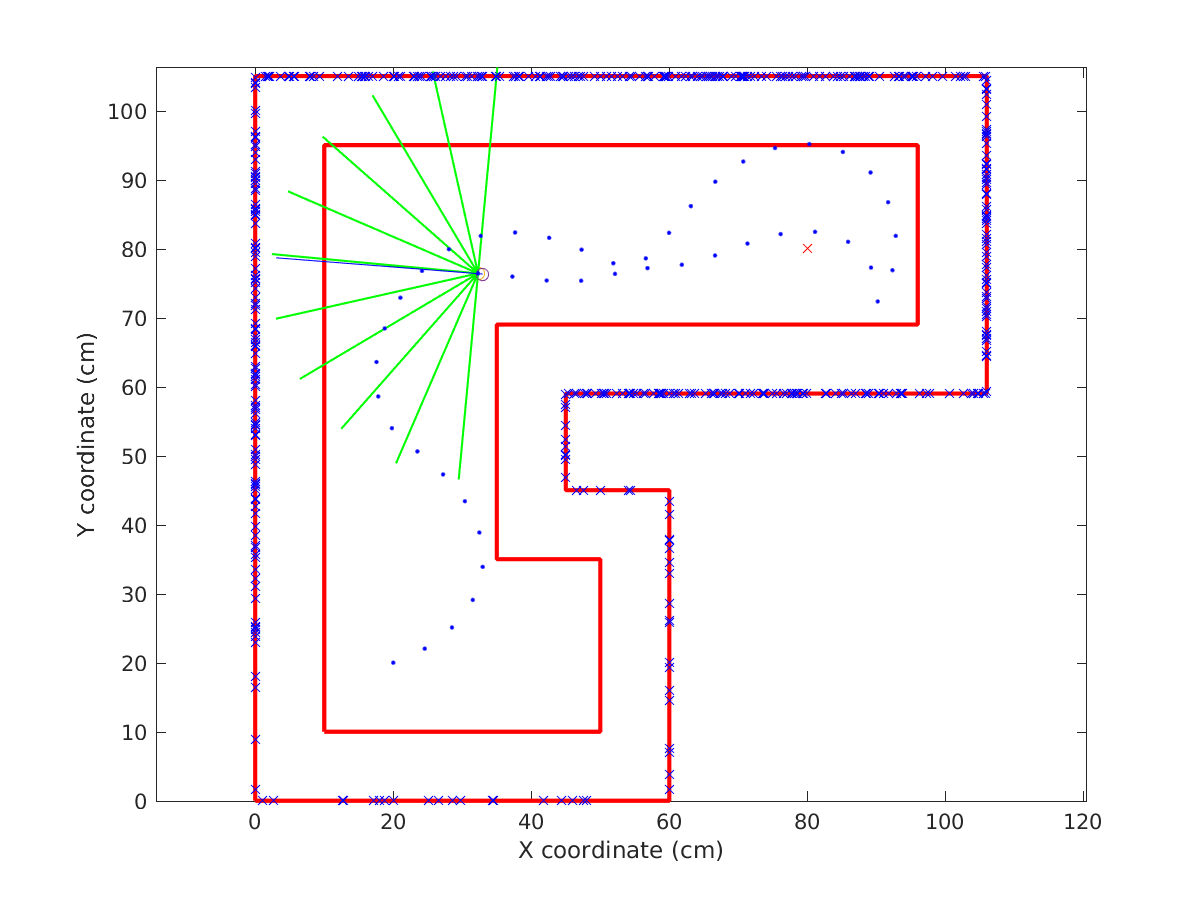
\includegraphics[width=.75\textwidth]{apf3}
			
			\caption{Combined exploration (artificial potential field with $\epsilon=0.2$ and collision avoidance), the former explores the space, a latter makes sure that the robot does not collide with the wall in any circumstances.}
			\label{fig:apf3}
	 	\end{figure}
	 	
	\subsubsection{Path planning} 	
	
		After the PFL is converged, the robot can plan its path from its current location to the target. The planning algorithm was a standard A* search \parencite{introduction_astar} on a visibility graph \parencite{choset_principles_2005} defined by the map, robot and target. This way the search space for the optimal path is greatly reduced and the movements are smoother compared to a grid-word representation. Figure \ref{fig:vm1} shows the visibility graph with the optimal path between the robot and the target.
		
		\begin{figure}[h]
		    \centering
  	 		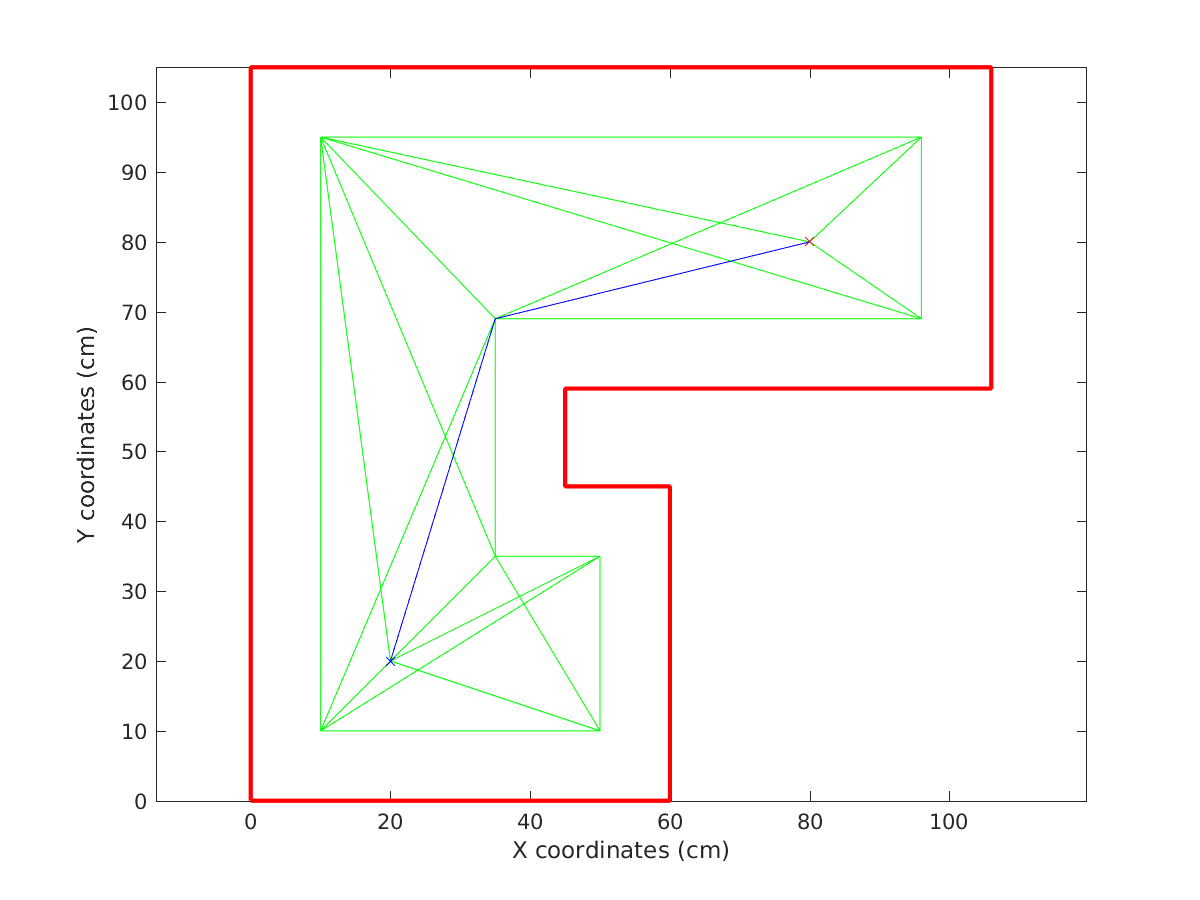
\includegraphics[width=.75\textwidth]{vm1}
		    \caption{A* search on the visibility graph finds the shortest path (blue line) between the robot and the target (blue and red cross respectively). The modified map is used, so the robot does not go closer to the walls than 10cm.}
		    \label{fig:vm1}
	 	\end{figure}
	 	
		\FloatBarrier
 	
 	\section{Results} \label{sec:result}
 	
 		\subsection{Simulation}
\begin{table}[h]
\begin{center}
	\begin{tabular}{ |c|c|c|c| }
		\hline
		Map & \multicolumn{1}{|p{3cm}|}{\centering Avg. completition time(s) } &\multicolumn{1}{|p{3cm}|}{\centering Avg. distance from target(cm) }  & collision(\%)  \\ 
		\hline
		\hline
		1 & 5.33 & 0.67 & 0 \\  
		2 & 8.01 & 0.57 & 0 \\ 
		3 & 14.74 & 1.03 & 0 \\ 
		\hline 
	\end{tabular}
	\caption{Results without noise}
	\label{table:nonoise}
\end{center}
\end{table}

\begin{table}[h]
\begin{center}
	\begin{tabular}{ |c|c|c|c| }
		\hline
		Map & \multicolumn{1}{|p{3cm}|}{\centering Avg. completition time(s) } &\multicolumn{1}{|p{3cm}|}{\centering Avg. distance from target(cm) }  & collision(\%)  \\ 
		\hline
		\hline
		1 & 2.81 & 0.25  & 0 \\  
		2 & 3.63 & 0.35  & 0 \\ 
		3 & 10.08 & 5.17  & 0 \\ 
		\hline 
	\end{tabular}
	\label{table:noise}
	\caption{Results with noise on sensor ($\pm$2 cm), motion ($\pm$0.01 cm), turning ($\pm$0.0001 rad)}
\end{center}
\end{table}

Table 1 and 2 show the results obtained after running the simulation 20 times each, with and without noise. As seen, the average competition time is improved in the second table adding noise, which helps the robot to reduce the time and distance from the target. 

In order to avoid collisions an important feature to set is the distance to recreate the map, these tests where conducted with a distance of 10 cm, other tests where conducted with a distance less than 5 having a collision percentage lower than 2\%. Later in the discussion section we will talk about the variable setting differences between the simulation and the real robot. 

\FloatBarrier
 		
		\subsection{Experiments}

	To test the performance of the robot it was tested in a physical setup. On top of the modelled noise there was also considerable false ultrasonic sensor readings due to the low angle between the sensor ray and the walls, which made the navigation harder,see Figure \ref{fig:scan1}, and also the time required to make the movement made the whole process slower. 
	
	The time it takes to get to a random target point on the map is typically between 53-180s depending on the starting point. A simple signal conditioning.
	
		\begin{figure}[h]
			\centering
			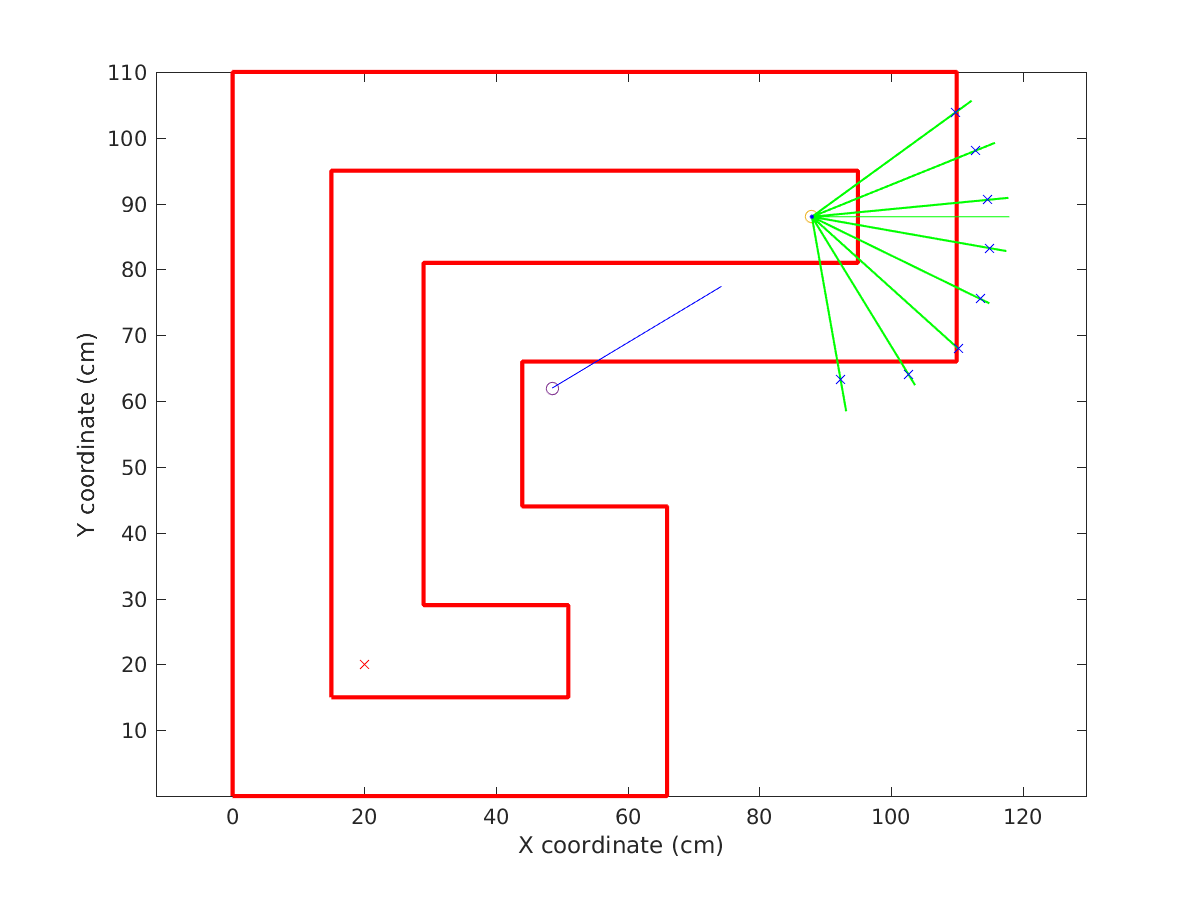
\includegraphics[width=\textwidth]{scan1}
			\caption{Sensor scanning beams showing the error between the perception of the robot and the map}
			\label{fig:scan1}
		\end{figure}
		
 		
 	\section{Discussion} \label{sec:discuss}
 
	 We achieved the objectives of designing and modelling a mobile robot, implementing a particle-filters algorithm for addresing the kidnapping robot problem and implementing an A* graph search algorithm for navigating the robot towards a goal. On the design stage, we addressed the challenges on how to build the robot for navigating  'smoothly' on a imperfect environment (not uniform floor, not continums walls, etc). We learned how to select an adequate number of particles and choose a proper number of beams for the sensor reading through simulated experiments, additionally we developed an exploring algorithm instead of a random exploration, in seeks for an accurate and fast localisation; for the robot navigation, using purely A* graph was not enough, we further developed an algorithm (i.e. map resizing) for keeping the robot as being centered as possible within the map.

%The difference between the simulation and the real robot 
 
 \printbibliography
 
% \section*{Appendix}
 
 		 	
	 	
\end{document}

